\subsection{Clustering}
\label{Res_Clu}

Using the simpleKMeans clustering algorithm in Weka results in the graph in figure \ref{fig:clusters}. The x-axis is the name of the country, the y-axis is the year and the color of the cross is the cluster the country belongs to at that time. The centroids of the clusters can be seen in the appendix REFERENCE!!!!!!

\begin{figure}[h!]
  \centering
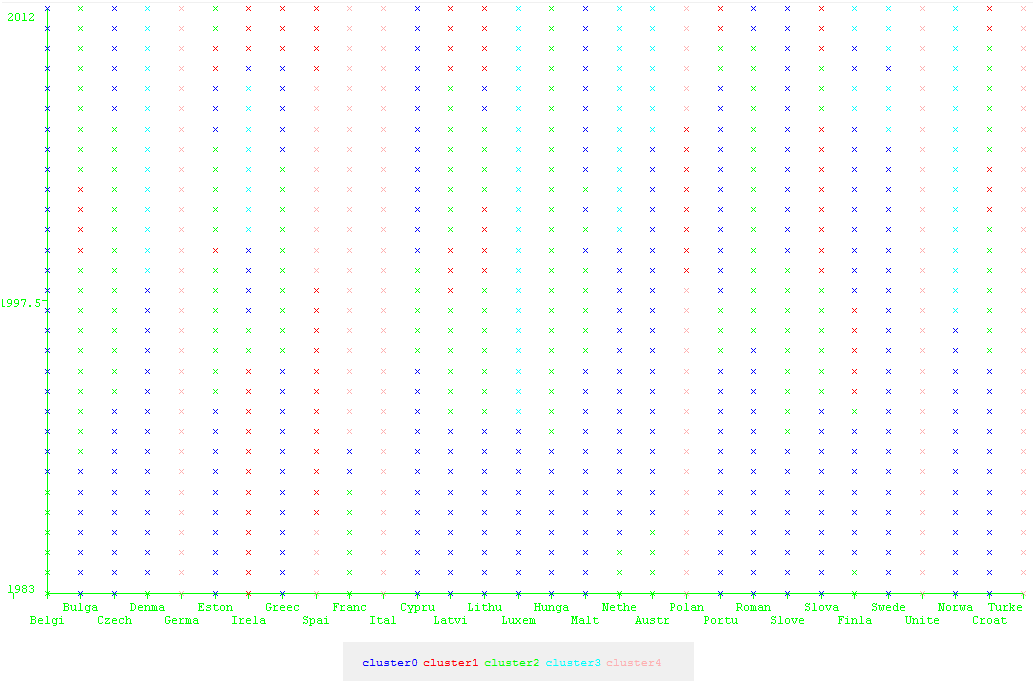
\includegraphics[width=\textwidth]{Appendix/Images/kMeans}
\caption{Graphical representation of what clusters the countries belong to at what year}
\label{fig:clusters}
\end{figure}

Looking at the graph, there are four countries that never change cluster: Germany, Italy, United Kingdom and Turkey. Furthermore, they are in the same category